\chapter{后处理技术与方法的扩展}
\label{chap:caa}

在本章中我们讨论将本文中介绍的流体仿真技术应用至不同领域时,一些值得注意的要点,及所需的一些后处理技术。

\section{应用于视觉动画时的仿真需求及后处理}
在视觉动画中,我们主要需求真实感的烟雾渲染。而这一过程所需的烟雾数据一般为烟雾的密度场 (表示各个位置烟雾的浓淡),而我们通过仿真得到的是流体的速度场,这自然需要模拟一个烟雾的传播 (advection) 过程。比较常见的传播方法是欧拉方法,即基于网格的。但是这有诸多的问题,其中最重要的一点是湍流仿真中有非常多的高频信号,而网格的空间采样频率很难捕捉到这些信号~\cite{bridson2015fluid},以至于传播得到的烟雾十分平滑,失去湍流的特征。而粒子则不受这一限制。对于一个被传播的物理量$q$,粒子的传播方程$Dq/Dt=0$表明粒子上所携带的值不会受到任何的滤波或信息丢失,十分适合我们的需求。所以我们在这里介绍一种通过粒子与网格的混合方法生成烟雾密度场的方法。该方法主要分为三个部分:粒子的生成、粒子的传播、粒子到网格的转换。

\paragraph{粒子的生成}
首先,我们先在场中确定一块区域,作为粒子的发射端。我们需要对该区域进行采样以真正决定粒子的初始位置。出于不同的需求,可能该区域不同位置的初始烟雾密度会不同,那么我们需要根据密度来进行采样。假如密度是均匀的,我们只需要进行均匀的随机采样。接下来我们要考虑一次性注入与连续注入两种情况。如果是一次性注入,我们只需要确定场中存在的粒子数量$N$,并一次性采样完毕,进行传播得到烟雾的动态。而连续注入时一个需要被确定的量是发射速率 (emission rate) $dN/dt$。即每一个时间步长,我们都应该发射$n=\Delta t dN/dt$个粒子。我们要注意的是,连续注入时需要避免每个时间步长粒子的初始化位置相同的情况。那样会形成多条脉线 (streakline),而不是形成一个烟雾一样的连续体。

此外,还有一个问题是,在连续注入时,如果我们在仿真每一帧的开始注入固定量的粒子,令其随速度场传播,当速度足够快时,我们会看到一团团离散的烟雾,这非常影响视觉效果 (见图~\ref{img:smoke_particles})。为了解决这一问题,我们可以给每个粒子一个随机的生成时间,这个随机时间来源于在一个时间步长$dt$内的均匀分布。之后每个粒子只会沿着速度场传播剩余的时间,以达到真正的位置。

\begin{figure}[htb]
  \centering
    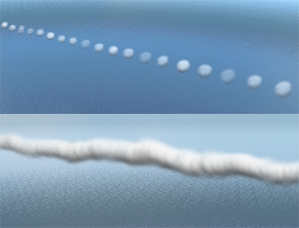
\includegraphics[width=0.7\columnwidth]{figures/smoke_particles.png}
  \bicaption[粒子传播时的不连续问题]{粒子传播时的不连续问题。在粒子相隔固定时间步长注入,且速度场中速度较快时,会出现不连续的烟雾团 (上图),而将粒子的生成时间随机化,可以避免这一问题 (下图)。}{Discontinuous proplem when advecting density using particles. If particles are emitted with fixed time interval and the velocities are fast, there will be discrete puffs moving through space (upper), while randomizing the emission time of particles can prevent the problem (bottom).}
  \label{img:smoke_particles}
\end{figure}

\paragraph{粒子的传播}
粒子的传播是影响精度的核心操作。在这一过程中我们需要求解一个微分方程来确定粒子的位置:
\begin{equation}
    \frac{d \mathbf{x}}{d t}=\mathbf{u}(\mathbf{x}),
    \label{eq:momentum_ode}
\end{equation}
其中$\mathbf{x}$为粒子的位置,$\mathbf{u}(\mathbf{x})$为速度场中$\mathbf{x}$点的速度。如果我们将离散的时间序列中第$n$个时刻记为$t^n$,此时的粒子位置记为$\mathbf{x}^{n}=\mathbf{x}(t^{n})$,而时间步长则为$\Delta t=t^{n+1}-t^{n}$,公式~\ref{eq:momentum_ode} 所表达的方程的初始条件为$\mathbf{x}(0)=\mathbf{x}^{0}$。则待求的解可以通过如下积分求得:
\begin{equation}
    \mathbf{x}(t)=\int_{0}^{t} \, \mathbf{u}(\mathbf{x}(\tau)) \, \mathrm{d}\tau.
\end{equation}

求解该方程最简单也是代价最小的时间积分方法即为前向欧拉 (forward Euler) 方法:
$\mathbf{x}^{n+1}=\mathbf{x}^{n}+\Delta t \mathbf{u}(\mathbf{x}^{n})$,
然而该方法只有一阶的精度。在时间步长不够小时,这一方法会带来很大的误差。而这一误差会随时间累积,最终使数值解与真实解偏差巨大。更精准的时间积分方法,如龙格-库塔 (Runge-Kutta,RK) 方法,可以得到更高阶精度的解。如二阶精度的龙格-库塔方法 (RK2) 可以写作
\begin{align}
    \begin{split}
    \mathbf{x}^{n+1 / 2} & =\mathbf{x}^n+\frac{1}{2} \Delta t \, \mathbf{u}\left(\mathbf{x}^n\right), \\
    \mathbf{x}^{n+1} & =\mathbf{x}^n+\Delta t \, \mathbf{u}\left(\mathbf{x}^{n+1 / 2}\right) .
\end{split}
\label{eq:2nd_rk}
\end{align}
而三阶精度的龙格-库塔方法 (RK3) 可以写作
\begin{align}
    \begin{split}
k_1 & =\mathbf{u}\left(\mathbf{x}^n\right), \\
k_2 & =\mathbf{u}\left(\mathbf{x}^n+\frac{1}{2} \Delta t \, k_1\right), \\
k_3 & =\mathbf{u}\left(\mathbf{x}^n+\frac{3}{4} \Delta t \, k_2\right), \\
\mathbf{x}^{n+1} & =\mathbf{x}^n+\frac{2}{9} \Delta t \, k_1+\frac{3}{9} \Delta t \, k_2+\frac{4}{9} \Delta t \, k_3 .
    \end{split}
    \label{eq:3rd_rk}
\end{align}
我们注意在公式~\ref{eq:2nd_rk} 与~\ref{eq:3rd_rk} 中,我们都忽略了速度场随时间的变化,这也导致这样的求解在时间上的精度仅为一阶的,但是我们在空间上可以获得更高的精度。

当然我们还要考虑一些特殊的情况,如在物体边界处的流体速度是非常低的。此时粒子很可能会以非常低的速度运动,或者在极端情况下粘滞在物体上。此外,即使我们使用了RK3方法,也依然可能受到时间步长的影响获得不精确的解,此时烟雾有可能穿过物体进入物体内部,造成视觉上的失真。为了处理这些问题,我们可以对粒子施加一个额外的惩罚力,惩罚力的大小与粒子距离物体边界的远近有关系,方向为远离物体的方向。可以抽象地认为,在粒子距离物体边界足够近的时候,物体会对粒子施加一个排斥力,拒绝粒子过度接近物体边界,甚至穿过物体边界。虽然这样做一定程度影响了粒子传播的精度,但这可以视为一个经验性的防止出现视觉失真现象的方法。

\paragraph{粒子到网格的转换}
我们使用粒子生成烟雾的目的,是为了制作视觉动画 (渲染)。虽然粒子也可以被直接渲染,但是庞大的粒子数量对高渲染效率造成很大挑战。而成熟的渲染管线更多采用基于网格的数据,许多全局光照以及动态效果也可以在基于网格的数据上做得更好。所以我们这里要讨论如何将粒子采样点转换回网格数据。

我们假设每一个粒子对烟雾密度的贡献为$s$,在最简单的情况下我们可以假设$s$对于所有粒子都是同一个值。然而基于不同的视觉效果,我们可以假设例如$s$是随时间递减的,而当$s$低于某一阈值后被视为消失 (即被删除)。假设对于粒子p,它的位置为$\mathbf{x}_p$,对烟雾密度的贡献为$s_p$。而对于网格的格点,每个点的位置为$\mathbf{x}_{i,j,k}$,其中$i$、$j$、$k$分别表达该点在网格中的坐标索引。这里$\mathbf{x}_{i,j,k}$与$\mathbf{x}_p$处于同一空间。则每个格点上的烟雾密度可以记为
\begin{equation}
    s_{i,j,k}=\sum_p s_p \, K(\mathbf{x}_p-\mathbf{x}_{i,j,k}).
    \label{eq:particle_sijk}
\end{equation}
在公式~\ref{eq:particle_sijk} 中$K$是一个核函数 (kernel function),这里该函数的具体形式没有严格的要求,举例来说我们可以使用二次B样条 (quadratic B-spline) 来进行构造:
\begin{align}
\label{eq:particle_kernel}
& k(x, y, z)= h\left(\frac{x}{\Delta x}\right) h\left(\frac{y}{\Delta x}\right) h\left(\frac{z}{\Delta x}\right), \\
& \quad h(r)=\left\{\begin{array}{cl}
\frac{1}{2}\left(r+\frac{3}{2}\right)^{2} & ,-\frac{3}{2} \leq r<-\frac{1}{2}, \\
\frac{3}{4}-r^{2} & ,-\frac{1}{2} \leq r<\frac{1}{2}, \\
\frac{1}{2}\left(\frac{3}{2}-r\right)^{2} & ,\frac{1}{2} \leq r<\frac{3}{2}, \\
0 & : \text { 其他情况, }
\end{array}\right.
\end{align}
其中$\Delta x$是网格的大小。公式~\ref{eq:particle_kernel} 中对网格大小做了自适应处理,使得每个粒子对周边的网格格点的贡献是适当的,而不会使烟雾过度模糊或颗粒化。

\section{应用于物理量计算时的仿真需求及后处理}
在使用流体仿真进行物理量 (如升力系数、阻力系数、物体表面压力系数等) 计算时,为了尽可能地提升仿真的物理精度,在仿真时应注意以下几点:
\begin{itemize}
    \item 仿真域:由于目前的仿真域边界条件无法完美地模拟开放边界条件 (open boundary condition),即所有的仿真域边界都会对域内的流体产生影响,所以为了进一步减轻这一影响,通常仿真域在各个维度的大小应设置为物体的6-12倍;
    \item 网格分辨率:为了保证精度,一般网格大小$\Delta x$的尺度在物体特征长度的1000分之1左右。显然在这种分辨率下,单分辨率网格是不现实的,所以需要采用多分辨率网格;
    \item 网格构建:网格的构建应保证关键的结构和区域有足够的分辨率,如靠近物体边界的区域和物体的尾流区域。其中一些特殊结构需要额外加密,如细密格栅结构或曲率较大的结构。
  \end{itemize}

  \begin{figure}[htb]
    \centering
        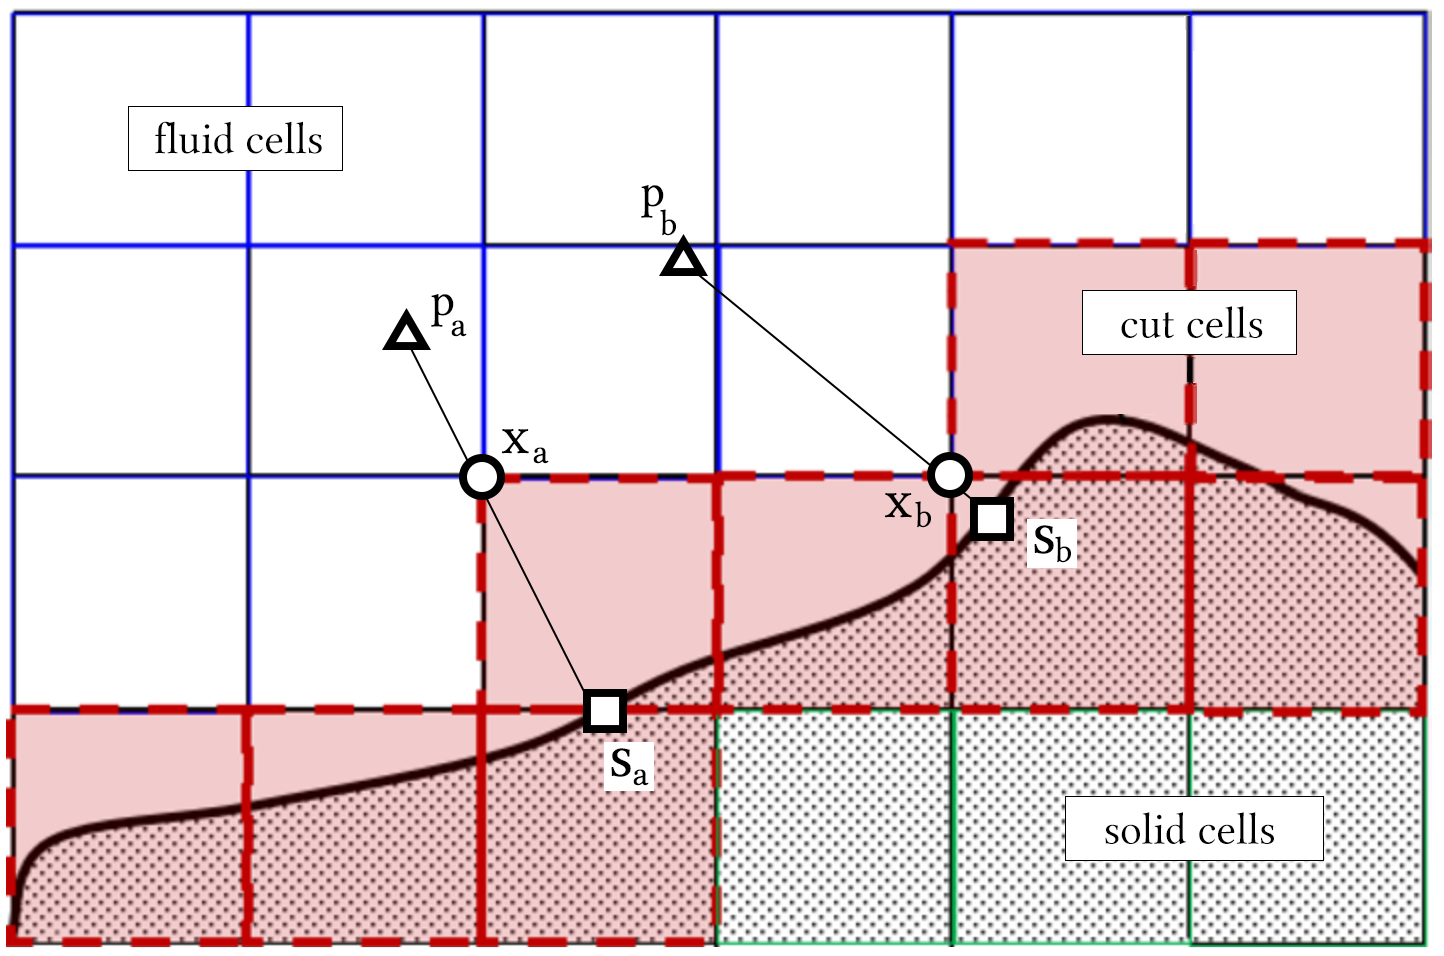
\includegraphics[width=0.95\columnwidth]{figures/pressure_projection.png}
    \bicaption[物体表面压力投影的示意图]{物体表面压力投影的示意图。图中蓝色网格为流体网格,红色为切削网格,绿色为固体网格,加点的区域为固体覆盖的区域。对于物体表面上的$s_a$与$s_b$点,如果直接从流体网格点插值物理量,则$x_a$与$x_b$点分别有着最大的影响。然而因为$x_a$与$x_b$点到物体边界的距离差别较大,这两个点的物理量也会有很大区别,造成物体表面物理量的不连续。而沿着$s_a$与$s_b$点法向向外走一定距离后,分别从$p_a$与$p_b$点插值物理量,可以减轻这一问题。}{Schematics of surface pressure projection. The blue, red and green cells in the firgue represent fluid, cut and solid cells, respectively. The dotted area is covered by solid object. For point $s_a$ and $s_b$ on object surface, if the physical quantities are directly interpolated from the nodes, node $x_a$ and $x_b$ would have the biggest impact, respectively. However, since node $x_a$ and $x_b$ have different distance to the object surface, resulting in largely different physical quantities which is discontinuous on surface. While interpolating from $p_a$ and $p_b$, which are points away from surface along their normals with a fixed distance can lift the problem.}
    \label{img:pressure_projection}
  \end{figure}

\section{应用于气动声学分析时的仿真需求及后处理}